
\documentclass{beamer}

% \usetheme{Frankfurt}
\usetheme{Malmoe}


\title{Multi-Objective taxi ride sharing}

\author{Diego D. Charrez Ticona\inst{1}}

\institute[National University of St Agustin]
{
  \inst{1}%
  Department of Computer Science\\
  National University of St Agustin
}

\date{Bio-inspired Computing, 2018}

\subject{Bio-inspired Computing}

\AtBeginSubsection[]
{
  \begin{frame}<beamer>{Outline}
    \tableofcontents[currentsection,currentsubsection]
  \end{frame}
}

\begin{document}

\begin{frame}
  \titlepage
\end{frame}

\begin{frame}{Outline}
  \tableofcontents
\end{frame}


\section{Introduction} %----------------------------------------

\subsection{Problem}

\begin{frame}{Problem}{}
    The problem models this situation:
  \begin{itemize}
  \item { N people are located in the same origin. }
  \item { They decide to ride to different location sharing taxis. }
  \item { Taxi assignment must be done in order to minimize the total cost of the passengers. }
  \end{itemize}
\end{frame}

\subsection{Restrictions}
\begin{frame}{Restrictions}{}
  \begin{itemize}
  \item { Each taxis has a limited number of passengers. }
  \item { The max number of taxis to N passengers is N }
  \item { Cost is given by the initial cost and the distance traveled. }
  \item { Each taxi has a limited number of passengers. }
  \end{itemize}
\end{frame}

\subsection{Example}
\begin{frame}{Example}{}
The objective is to minimize the total cost of all passengers and the perceived delay by the passengers to arrive to their destinations:
  \begin{figure}
      \centering
      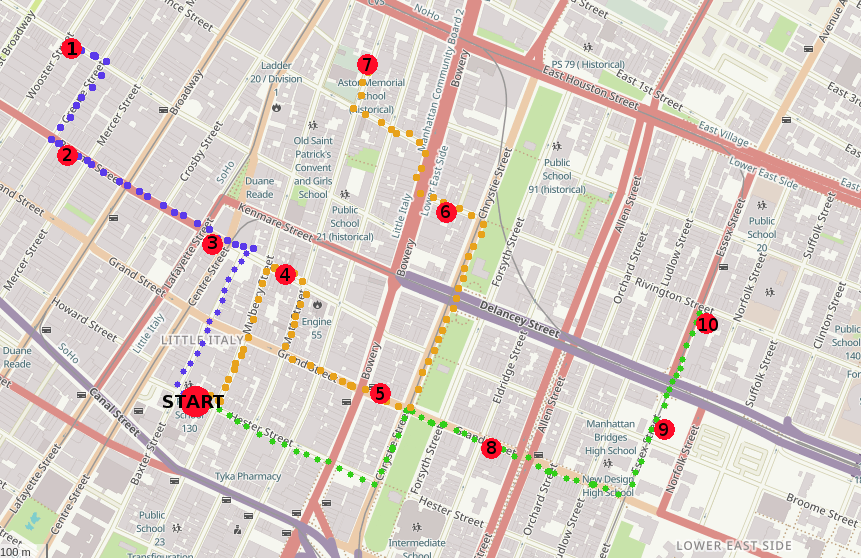
\includegraphics[scale=0.36]{imgs/example.png}
      \caption{Taxi ride sharing}
      \label{fig:example}
  \end{figure}
\end{frame}

\section{Implementation} %----------------------------------------

\subsection{Input values}
\begin{frame}{Input values}{}
\begin{itemize}
    \item Number of passengers.
    \item An array with indicating if a passenger is able to wait.
    \item An array of taxis with their capacities.
    \item Initial cost.
    \item Cost's matrix between all points.
    \item Traveled time's matrix between all points.
\end{itemize}
\end{frame}

\subsection{Codification}
\begin{frame}{Codification}{}
Passengers between zeros represent that are in the same taxi.
  \begin{figure}
      \centering
      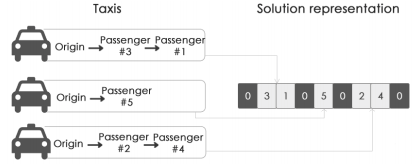
\includegraphics[scale=0.36]{imgs/codification.png}\\[-1ex]
       {\tiny Source: Multiobjective taxi sharing optimization using the NSGA-II evolutionary algorithm }
      \caption{Representation of taxi ride sharing problem}
      \label{fig:example}
  \end{figure}
\end{frame}


\appendix
\section<presentation>*{\appendixname}
\subsection<presentation>*{For Further Reading}

\begin{frame}[allowframebreaks]
  \frametitle<presentation>{For Further Reading}
    
  \begin{thebibliography}{10}
    
  \beamertemplatebookbibitems
  % Start with overview books.

  \bibitem{Author1990}
    A.~Author.
    \newblock {\em Handbook of Everything}.
    \newblock Some Press, 1990.
 
    
  \beamertemplatearticlebibitems
  % Followed by interesting articles. Keep the list short. 

  \bibitem{Multiobjective evolutionary algorithms for the taxi sharing problem}
    Massobrio, Renzo
    \newblock {\em International Journal of Metaheuristics}, 5(1):67--90,
    2016.
  \end{thebibliography}
\end{frame}

\end{document}


